% GNUPLOT: LaTeX picture with Postscript
\begingroup
  \fontfamily{Serif}%
  \selectfont
  \makeatletter
  \providecommand\color[2][]{%
    \GenericError{(gnuplot) \space\space\space\@spaces}{%
      Package color not loaded in conjunction with
      terminal option `colourtext'%
    }{See the gnuplot documentation for explanation.%
    }{Either use 'blacktext' in gnuplot or load the package
      color.sty in LaTeX.}%
    \renewcommand\color[2][]{}%
  }%
  \providecommand\includegraphics[2][]{%
    \GenericError{(gnuplot) \space\space\space\@spaces}{%
      Package graphicx or graphics not loaded%
    }{See the gnuplot documentation for explanation.%
    }{The gnuplot epslatex terminal needs graphicx.sty or graphics.sty.}%
    \renewcommand\includegraphics[2][]{}%
  }%
  \providecommand\rotatebox[2]{#2}%
  \@ifundefined{ifGPcolor}{%
    \newif\ifGPcolor
    \GPcolortrue
  }{}%
  \@ifundefined{ifGPblacktext}{%
    \newif\ifGPblacktext
    \GPblacktexttrue
  }{}%
  % define a \g@addto@macro without @ in the name:
  \let\gplgaddtomacro\g@addto@macro
  % define empty templates for all commands taking text:
  \gdef\gplbacktext{}%
  \gdef\gplfronttext{}%
  \makeatother
  \ifGPblacktext
    % no textcolor at all
    \def\colorrgb#1{}%
    \def\colorgray#1{}%
  \else
    % gray or color?
    \ifGPcolor
      \def\colorrgb#1{\color[rgb]{#1}}%
      \def\colorgray#1{\color[gray]{#1}}%
      \expandafter\def\csname LTw\endcsname{\color{white}}%
      \expandafter\def\csname LTb\endcsname{\color{black}}%
      \expandafter\def\csname LTa\endcsname{\color{black}}%
      \expandafter\def\csname LT0\endcsname{\color[rgb]{1,0,0}}%
      \expandafter\def\csname LT1\endcsname{\color[rgb]{0,1,0}}%
      \expandafter\def\csname LT2\endcsname{\color[rgb]{0,0,1}}%
      \expandafter\def\csname LT3\endcsname{\color[rgb]{1,0,1}}%
      \expandafter\def\csname LT4\endcsname{\color[rgb]{0,1,1}}%
      \expandafter\def\csname LT5\endcsname{\color[rgb]{1,1,0}}%
      \expandafter\def\csname LT6\endcsname{\color[rgb]{0,0,0}}%
      \expandafter\def\csname LT7\endcsname{\color[rgb]{1,0.3,0}}%
      \expandafter\def\csname LT8\endcsname{\color[rgb]{0.5,0.5,0.5}}%
    \else
      % gray
      \def\colorrgb#1{\color{black}}%
      \def\colorgray#1{\color[gray]{#1}}%
      \expandafter\def\csname LTw\endcsname{\color{white}}%
      \expandafter\def\csname LTb\endcsname{\color{black}}%
      \expandafter\def\csname LTa\endcsname{\color{black}}%
      \expandafter\def\csname LT0\endcsname{\color{black}}%
      \expandafter\def\csname LT1\endcsname{\color{black}}%
      \expandafter\def\csname LT2\endcsname{\color{black}}%
      \expandafter\def\csname LT3\endcsname{\color{black}}%
      \expandafter\def\csname LT4\endcsname{\color{black}}%
      \expandafter\def\csname LT5\endcsname{\color{black}}%
      \expandafter\def\csname LT6\endcsname{\color{black}}%
      \expandafter\def\csname LT7\endcsname{\color{black}}%
      \expandafter\def\csname LT8\endcsname{\color{black}}%
    \fi
  \fi
  \setlength{\unitlength}{0.0500bp}%
  \begin{picture}(12960.00,8640.00)%
    \gplgaddtomacro\gplbacktext{%
      \csname LTb\endcsname%
      \put(1100,640){\makebox(0,0)[r]{\strut{} 16000}}%
      \csname LTb\endcsname%
      \put(1100,1380){\makebox(0,0)[r]{\strut{} 18000}}%
      \csname LTb\endcsname%
      \put(1100,2120){\makebox(0,0)[r]{\strut{} 20000}}%
      \csname LTb\endcsname%
      \put(1100,2860){\makebox(0,0)[r]{\strut{} 22000}}%
      \csname LTb\endcsname%
      \put(1100,3600){\makebox(0,0)[r]{\strut{} 24000}}%
      \csname LTb\endcsname%
      \put(1100,4340){\makebox(0,0)[r]{\strut{} 26000}}%
      \csname LTb\endcsname%
      \put(1100,5079){\makebox(0,0)[r]{\strut{} 28000}}%
      \csname LTb\endcsname%
      \put(1100,5819){\makebox(0,0)[r]{\strut{} 30000}}%
      \csname LTb\endcsname%
      \put(1100,6559){\makebox(0,0)[r]{\strut{} 32000}}%
      \csname LTb\endcsname%
      \put(1100,7299){\makebox(0,0)[r]{\strut{} 34000}}%
      \csname LTb\endcsname%
      \put(1100,8039){\makebox(0,0)[r]{\strut{} 36000}}%
      \csname LTb\endcsname%
      \put(1734,440){\makebox(0,0){\strut{} 2000}}%
      \csname LTb\endcsname%
      \put(2763,440){\makebox(0,0){\strut{} 2002}}%
      \csname LTb\endcsname%
      \put(3792,440){\makebox(0,0){\strut{} 2004}}%
      \csname LTb\endcsname%
      \put(4821,440){\makebox(0,0){\strut{} 2006}}%
      \csname LTb\endcsname%
      \put(5850,440){\makebox(0,0){\strut{} 2008}}%
      \csname LTb\endcsname%
      \put(6878,440){\makebox(0,0){\strut{} 2010}}%
      \csname LTb\endcsname%
      \put(7907,440){\makebox(0,0){\strut{} 2012}}%
      \csname LTb\endcsname%
      \put(8936,440){\makebox(0,0){\strut{} 2014}}%
      \put(-10,4339){\rotatebox{-270}{\makebox(0,0){\strut{}Full--Time Employee Earnings}}}%
      \put(280,4339){\rotatebox{-270}{\makebox(0,0){\strut{}(median per employee per annum, gross GBP$\pounds$, not adjusted)}}}%
      \put(5078,-70){\makebox(0,0){\strut{}Year}}%
      \put(5078,8539){\makebox(0,0){\strut{}Regional Employee Earnings (gross annual)}}%
    }%
    \gplgaddtomacro\gplfronttext{%
      \csname LTb\endcsname%
      \put(12056,7889){\makebox(0,0)[r]{\strut{}United Kingdom (Whole)}}%
      \csname LTb\endcsname%
      \put(12056,7589){\makebox(0,0)[r]{\strut{}England (Whole)}}%
      \csname LTb\endcsname%
      \put(12056,7289){\makebox(0,0)[r]{\strut{}North--East England}}%
      \csname LTb\endcsname%
      \put(12056,6989){\makebox(0,0)[r]{\strut{}North--West England}}%
      \csname LTb\endcsname%
      \put(12056,6689){\makebox(0,0)[r]{\strut{}Yorkshire and The Humber}}%
      \csname LTb\endcsname%
      \put(12056,6389){\makebox(0,0)[r]{\strut{}East Midlands}}%
      \csname LTb\endcsname%
      \put(12056,6089){\makebox(0,0)[r]{\strut{}West Midlands}}%
      \csname LTb\endcsname%
      \put(12056,5789){\makebox(0,0)[r]{\strut{}East England}}%
      \csname LTb\endcsname%
      \put(12056,5489){\makebox(0,0)[r]{\strut{}London}}%
      \csname LTb\endcsname%
      \put(12056,5189){\makebox(0,0)[r]{\strut{}South--East England}}%
      \csname LTb\endcsname%
      \put(12056,4889){\makebox(0,0)[r]{\strut{}South--West England}}%
      \csname LTb\endcsname%
      \put(12056,4589){\makebox(0,0)[r]{\strut{}Wales}}%
      \csname LTb\endcsname%
      \put(12056,4289){\makebox(0,0)[r]{\strut{}Scotland}}%
      \csname LTb\endcsname%
      \put(12056,3989){\makebox(0,0)[r]{\strut{}Northern Ireland}}%
    }%
    \put(9600,3300){\makebox(0,0)[l]{\strut{}\small UK Regional Employee Earnings}}%
    \put(9600,1700){\makebox(0,0)[l]{\strut{}\begin{minipage}[t][][t]{6.5cm}\small
Full--time median employee earnings (gross) per annum, not adjusted. Based on full--time employees receiving adult rates of pay. In this survey, full-time is defined to be more than 30 hours of paid work per week for all professions except teaching, for which more than 25 hours of paid work per week qualifies as full--time. Source: {\it Full-time employees' pay by work region, United Kingdom, April 1997--2014}, {\it Annual Survey of Hours and Earnings (ASHE)}, \textit{\it ONS}.
\end{minipage}}}%
    \gplbacktext
    \put(0,0){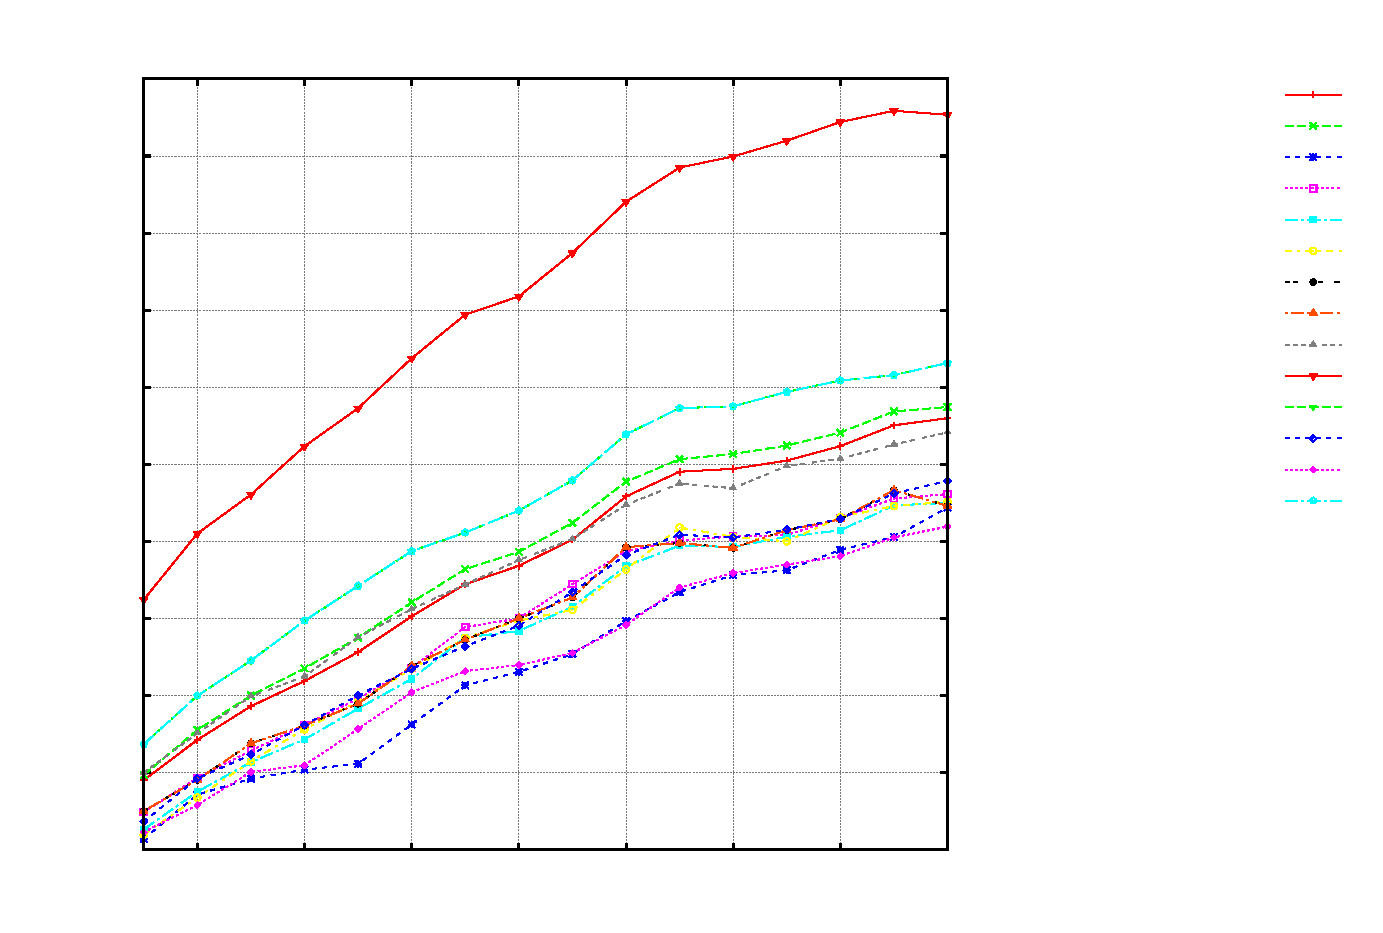
\includegraphics{./plots/regional/regional-rankings.eps}}%
    \gplfronttext
  \end{picture}%
\endgroup
